\documentclass{article} % article doctype, possible font size range from 8pt to 20pt with not all being avaiable.
\title{\huge Willy The Robot Project Plan}
\author{Jeroen van 't Hul\\S1139163  \and Thomas Zwaanswijk\\s1089273 \and Tom van den Noort\\s1101124}
\date{\parbox{\linewidth}{\centering%
	\today\endgraf\bigskip
	Supervisor \hspace*{3cm}	Main Stakeholder\endgraf\medskip
	Mischa Mol \hspace*{3cm} Ilja Clabbers\endgraf\medskip
	Windesheim Zwolle\endgraf}}

% include packages
\usepackage{graphicx}
\usepackage{caption}
\usepackage{mathabx}
\usepackage{wrapfig}
\usepackage{siunitx}
\usepackage[margin=1.0in]{geometry} % sets page margin, 2.0in is default.
\usepackage{titlesec}
%\usepackage{hyperref}
\usepackage{textcomp}
\usepackage{listings}
\usepackage[table,xcdraw]{xcolor}
\usepackage{float}
\usepackage[export]{adjustbox}
\usepackage{todonotes}
\usepackage{multirow}	% used for table multirow support
\usepackage[nottoc,numbib]{tocbibind} % Adds bibliography / references to TOC and numbers that section.

\usepackage{indentfirst}
\usepackage{eurosym}
\usepackage{listings}

\usepackage{array}
\usepackage{comment}
\usepackage{url}
\usepackage[breaklinks]{hyperref}
\usepackage{breakurl}


\def\UrlBreaks{\do\/\do-}


% ----- custom commands ----- %
% Wrapper for paragraph command. Forces newline after paragraph title
\newcommand{\myparagraph}[1]{\paragraph{#1}\mbox{}\\} % Without \mbox{} all newlines will be ignored, making the first sentence appear on the same line as a paragraph title.
% monospace codeblock
\def\code#1{\texttt{#1}}
% changing the ToC depth in the document enviroment
\newcommand{\changelocaltocdepth}[1]{%
	\addtocontents{toc}{\protect\setcounter{tocdepth}{#1}}%
	\setcounter{tocdepth}{#1}%
}


\newcolumntype{L}[1]{>{\raggedright\let\newline\\\arraybackslash\hspace{0pt}}m{#1}}
\newcolumntype{C}[1]{>{\centering\let\newline\\\arraybackslash\hspace{0pt}}m{#1}}
\newcolumntype{R}[1]{>{\raggedleft\let\newline\\\arraybackslash\hspace{0pt}}m{#1}}

\setcounter{tocdepth}{2} % only part,chapters,sections, subsections appear in ToC



\DeclareCaptionFormat{cancaption}{#1#2#3\par} % Normal format actually
\DeclareCaptionLabelFormat{cancaptionlabel}{#1}
\captionsetup[figure][number]{format=cancaption,labelformat=cancaptionlabel}
\graphicspath { {images/}{../images/} }

\begin{document}
\maketitle

\begin{figure}[H]
\centering
\includegraphics[width=12 cm]{WTRLogo.png}
\end{figure}
\thispagestyle{empty}
\newpage
\setcounter{page}{1}
\tableofcontents
\newpage

% Sections
\section{Introduction}
This research is meant to create an inventory of the current state of the movements WTR\ref{trm::WTR} is capable of performing.
In addition, this document contains a list of proposed improvements in order to increase the accuracy of the autonomous driving.
By creating a list of the range of movement WTR can perform and noting any defects or issues with those, it should become easier to create a proper list of improvements.
Several sections will deal with the sensors, how they benefit the robot and their mounting as well.
\newpage

\section{Project Summary}
This section contains an explanation of what Willy is meant to do, how the current project will work towards that goal, and to what ends.

Willy started its life as a concept for a garbage collecting robot, meant to drive autonomously through the city center in Zwolle.
For a few years the project continued with that as a goal, until Hogeschool Windesheim and TAoR (The Art of Robotics) went their separate ways \cite{taor}.
The project is now run solely by Windesheim.
According to the previous group, there is still some ongoing discussion about who truly owns the project, but for the sake of simplicity the assumption will be made Willy solely belongs to Windesheim.

After this falling out, Willy got a new purpose in its robotic life, as a robotic greeter.
The goal of Willy is now no longer to drive around and remind people to throw away their garbage neatly, but instead drive around and inform people about public events at Windesheim.

For the current project, this does not matter much.
The goal of this semester of Future Technology for Willy is to improve the autonomous driving to the point where the April tags (located on the ceiling of various points in T5) are no longer needed.

Initially, the assumption was made that these were used as key points in navigation for Willy, but after a very informative meeting with the previous group, it was revealed that the only reason these tags still exist is to use as calibration points and setting an easy target for Willy to navigate to.
This means that the scope of the project is slightly shifted.
As such, the key focus is on lessening the standard PID controller feedback swing (as illustrated in figure \ref{fig::pid}.

\begin{figure}[H]
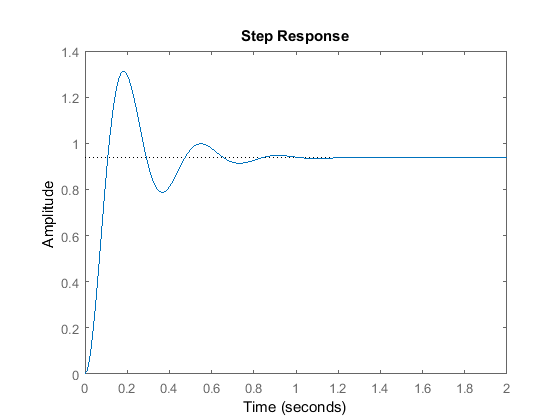
\includegraphics[width=12cm]{pidgraph.png}
\caption{A rough demonstration of PID correction}
\label{fig::pid}
\end{figure}

By reducing the amount of corrections needed by the navigation stack \cite{navstack}, the "Drunken Polish Driving" effect, as described by one of the previous project groups, can be lessened.
This would mean a smoother autonomous driving experience.
\newpage
\section{Motivation}
This chapter describes the motivation for the project. 
it described why it started, what the current problem is and the set goal to reach within the allotted time.

\subsection{Context}
Windesheim University wants to have a robot which can drive autonomously and interact with guests to provide them with information on open days.
Several project groups have been working on this goal prior to this project, creating and/or completing various modules that work together to realize the autonomy and interactivity of the robot.
The goal that this group wants to reach will be described below and continues from what the previous group(s) have left behind.

\subsection{Problem}
The main problem of the robot in its current state is the autonomous driving capabilities. 
The robot is able to drive autonomously to a certain degree, but it lacks a fluent and safe navigation system. 
Next to this the overall impression of the robot is messy. 
The cables are not properly managed, sensors and controllers are loosely attached. 
Mechanically the undercarriage is not stable and one wheel rubs against the frame. 
These and other flaws pose a potential safety risk to the robot and others nearby. 

\subsection{Goal}
Out of the problems stated above, autonomous driving has been chosen as the core focus of this project. 
The challenge is to improve upon the driving system(s) to make sure the robot will be able to drive autonomously without posing a threat to itself, the environment or others.
Currently, the scope is limited to T5 in Windesheim, but the ultimate end-goal is that Willy can be used anywhere without issue.
Additionally, the documentation of the project itself needs to be corrected and maintained, giving future groups the ability to pick up and continue the project without any delay or misunderstandings.

\subsection{History}
This is not the first project group to work on Willy.
At this point in time, there have been 4 other groups to work on the robot.
That means that there is a lot of pre-existing code and functionality, all of which must be considered and either re-worked or worked with.
Another curiosity is that Willy started off as a completely different product.
Originally, it started as a garbage collection robot, but somewhere during development of Willy the company responsible for Willy handed it over to Windesheim, who chose to turn Willy into a robot greeter to be used during public events.
As such, the choice was made to focus on autonomous driving, with as a sub-goal to reduce the clutter present on Willy and improve the way the sensors are mounted.

\subsection{Parties, Roles and Stakeholders}
Currently, the stakeholders are as follows:
\begin{center}
\begin{tabular}{|l|l|l|}
\hline
\textbf{Name} & \textbf{Role} & \textbf{Contact Info} \\ \hline
Mischa Mol 	& Product Owner/Coach & \href{mailto:mc.mol@windesheim.nl}{mc.mol@windehseim.nl} \\ \hline
Thomas Zwaanswijk & Project member & \href{mailto:thomas.zwaanswijk@windesheim.nl}{thomas.zwaanswijk@windesheim.nl} \\ \hline
Tom van der Noort & Project member & \href{mailto:tom.vanden.noort@windesheimflevoland.nl}{tom.vanden.noort@windesheimflevoland.nl} \\ \hline
Jeroen van `t Hul & Project leader & \href{jeroen.van.t.hul@windesheim.nl}{jeroen.van.t.hul@windesheim.nl} \\ \hline
\end{tabular}
\end{center}
\newpage

\section{Project}
In this chapter the project will be described in further detail, such as the scope and the deliverables.
\subsection{Scope}
Every task that will take the project group closer to the target goal can be considered something that is in scope of this project. 
This is something that can be considered a grey area in practice. 
It is not always that easy to know how relevant a certain task is, therefore the team needs to be alert that a certain task does not go out of scope. 
To help with this, the relevant goals of this project will be described below. 
\begin{itemize}
\item Safety for the robot and its surroundings
\item Improved autonomous driving
\item Mechanical improvements to the structure of the robot
\item Electrical improvements to the components of the robot
\item Well-maintained, simple documentation
\end{itemize}
Any tasks that do not contribute towards one of these goals is considered outside of the scope of the project to the discretion of the group.

\subsection{Deliverables}
\begin{itemize}
\item Project plan
\item Technical design document
\item Research report into current navigational abilities
\item Final report
\item Updated code \& Documents 
\end{itemize}

\newpage

\section{Methodology}
For this project, an agile methodology is very convenient.
There are of course multiple options when it comes to working in an agile manner, but as the entire group already has experience with SCRUM, that will be the method used.
The sprint duration will be two weeks, with daily stand-ups  being held every day.

\subsubsection{Daily Stand-up}
\label{sec::standup}
Every morning as soon as every member is present a stand-up will be held.
During this session every member tells the others what tasks they worked on yesterday, what tasks are going to be done today, as well as any anticipated challenges.
The purpose of this meeting is to ensure every member of the group knows what the others are doing, and allow them to offer accurate advice on current issues.

\subsubsection{Sprint review}
\label{sec::sprintrev}
A sprint review will be held at the end of every sprint, which means that this will be a bi-weekly event.
This should include a demonstration or presentation about the events that occurred in the last two weeks.
The product owner should be invited to every review, so that feedback from the product owner can be incorporated into the next sprint planning.

\subsubsection{Sprint Retrospective}
The retrospective offers the group a chance to consider what went well and what went poorly each sprint.
Therefore, this should be held after the review, but before the planning where possible.
The retrospective should be kept short and simple as much as possible, since after it the planning needs to be held.
The retrospective will be done through Trello, creating lists of what went well, what went poorly, and what helped along the way.
It ends when all cards have been discussed and any issues brought up have been resolved.

\subsubsection{Sprint Planning}
After every review, a sprint planning is held.
The goal of this is to select the tasks which have priority and move them to the appropriate sprint backlog. 
Any work that has not been finished is moved back to the backlog, and re-evaluated.
Any sprint planning beyond the first should start after the retrospective is done, preferably around noon, and finish at 4 o'clock.
After every feature has been discussed and supplied with story points, the planning is finished.
\newpage

\subsection{Daily \& Weekly Activities}
Certain activities are held on a regular basis.
These include the agile standards, weekly meetings and reports, as well as daily gatherings.

\subsubsection{Daily Stand-Up}
As has been mentioned before, a stand-up will be held every day.
They are described in section \ref{sec::standup}
\subsubsection{Weekly Meeting With Coach/Product Owner}
Especially at the beginning, it is important to meet with the coach Mischa Mol quite often, as a lot of work has already been done by previous teams.
In order to ensure that the main goal of the project is not missed, every week progress and difficulties can be discussed.
This allows feedback from the coach in addition to that given during the sprint review described in section \ref{sec::sprintrev}.

\subsection{Quality Management}
In order to ensure quality in both code and documentation, several measures have to be taken.

One of these is having to have at least one person review any code and documentation before it can be merged into a development branch.
This means that errors are more likely to be caught, since they are generally more obvious to people who did not write a section.

Another method that will be used is code standards. 
These can be found in appendix ~\ref{app::codecon}.

Code testing must be done by at least one person, who also then writes down the test results.
This allows for better transparency in what went wrong and why, resulting in easier bug-fixing.
\newpage

\subsection{Tools}
Not every tool will be supported in this project, as a lot of decisions have already been made by previous teams.

\begin{itemize}
\item Whatsapp - Communication within the team
\item GitHub - VC remote and reviews
\item Trello - Planning boards and reviews
\item Google Calendar  - Keeping track of meetings and planned absences
\item Robotic Operating System - The system used to control Willy, and what must be programmed in
\item UMLet - Free and open source tool for drawing diagrams, works well with GitHub for version control
\item Git - version control
\item MikTex - \LaTeX distribution for Windows
\item \LaTeX editor of choice - Note that only one member of the team has \LaTeX experience, and only in TexWorks
\item Google Drive - file sharing and places for keeping quick notes
\item Skylab - control of visuals of robot
\end{itemize}

\subsection{Agreements}
\begin{itemize}
	\item All code must follow the Google C++ Style where it is relevant and possible to do so.
	\item Branches can only be merged into development after at least one other member of the group has performed a code review and marked it as passing on Git.
	\item Code version control is done through GitHub
	\item Any work submitted must follow the Definition Of Done, or DoD.
\item General work days are from 9 to 4 where possible, with exception on mondays where PV subjects are concerned
\item The target amount of hours per week is 32 hours, regardless of their distribution throughout the week.
\item In case of late arrival, should there be unavoidable circumstances it can be ignored
\item Every time a group member is late due to their own fault, they must buy coffee for all group members.
\item After every third time, they must buy a treat of some description for the entire project group as well.
\item Communication is primarily done through Whatsapp or in person when available.
\end{itemize}
\newpage

\section{Schedule}
The following table describes the schedule of the project.
\begin{center}
\begin{tabular}{|l|l|}
\hline
\textbf{Week} & \textbf{Activities} \\ \hline
1: 28 January 2019 & Introduction \\ \hline
2: 4 February 2019 & Start sprint 0 \\ \hline
3: 11 February 2019 & Start sprint 1 \\ \hline
4: 18 February 2019 & Holiday \\ \hline
5: 25 February 2019 &  \\ \hline
6: 4 March 2019 & Start sprint 2 \\ \hline
7: 11 March 2019 &  \\ \hline
8: 18 March 2019 & Start sprint 3 \\ \hline
9: 25 March 2019 &  \\ \hline
10: 1 April  2019 & Start sprint 4 \\ \hline
11: 8 April 2019 &  \\ \hline
12: 15 April 2019 & Start sprint 5 \\ \hline
13: 22 April 2019 &  \\ \hline
14: 29 April 2019 & Start sprint 6 \\ \hline
15: 6 May 2019 &  \\ \hline
16: 13 May 2019 & Start sprint 7 \\ \hline
17: 20 May 2019 &  \\ \hline
18: 27 May 2019 & Start sprint 8 \\ \hline
19: 3 June 2019 &  \\ \hline
20: 10 June 2019 & Project deadline \\ \hline
\end{tabular}
\end{center}

\subsection{Global Sprint Planning}
\textbf{Sprint 0} \\
Introduction of the projects, team building, contacting stakeholders, project plan, contact with previous groups\\
\textbf{Sprint 1}\\
Getting to grips with Willy and ROS (Robotic Operating System)\\
\textbf{Sprint 2}\\
Functional design, mechanical design\\
\textbf{Sprint 3}\\
begin updating controls on Willy\\
\textbf{Spring 4}\\
work on Willy autonomous driving\\
\textbf{Sprint 5}\\
Continue autonomous driving\\
\textbf{sprint 6} \\
Continue autonomous driving\\
\textbf{sprint 7}\\
Testing\\
\textbf{Sprint 8}\\
Bugfixing + preparation for Winnovation \\

Any spare time will be dedicated to improving other features, but the scope of those is dependent of whether or not any time is left, and the interest of the group itself.
Additionally, the way Willy is currently built leaves a lot to be desired, so in any spare time improvements in the mounting of hardware and cable-management will also be made.

 \newpage

\section{Business Case}


\subsection{What Is The Problem?}
In its current iteration, Willy The Robot is capable of autonomous driving to some degree, but it is not yet capable of doing so fluently.
If Windesheim intends to use it as an automatic greeter, this would need to be improved, as it could cause a public incident by bumping into furniture or people.
The assignment of the current group is to find a way to correct the autonomous driving so that it can move around in safer manner.

\subsection{The Cost}
So far, the estimated base cost Windesheim is incurring by not out-sourcing Willy is around 40 hours for the coach, equivalent to about \euro 4000.
This does not include the cost of materials used for the production of Willy, which have already been invested.
For the task the current group has been assigned, several physical improvements could be used to correct the driving.

\begin{tabular}{|L{3cm}|L{6cm}|l|l|}
\hline
Solution		  & Summary 															  & Cost 	&Required Effort \\ \hline
Tank Steering & Replacing rear wheels with another set of wheels linked to main motors & High 	& High			\\ \hline
Single Rear Wheel & Replacing the two rear wheels with a single pivot wheel 		    	  & Low		& Low			\\ \hline
Single Bearing ball & Replacing the two rear wheels with a single ball in a fixture   & High  	& High			\\ \hline
Rotary Encoders on all wheels & Adding a small device to all wheels to count rotations & Med   	& Med			\\ \hline
Updating ROS movebase used & Updating code to use either custom software or pre-made which takes current frame into account & Free & High \\ \hline
\end{tabular}


Not all of these solutions would have equal results.
Tank steering, for example, would still mean that the ROS movebase\footnote{The movebase is the part of the code which translates instructions such as "turn right X degrees" into actual instructions for the motors} would need to be updated, but the end results would allow for a great range of movements, and a very small turning circle.
A small turning circle would be ideal for a crowded indoor event, such as Winnovation.
the single rear wheel solution would be cheap, as there are already wheels on the robot which could be re-purposed, but it would still require alterations to the frame of Willy, which would require materials as well.
However, it would mean that the turning circle would not be any smaller than in the current situation.
Alternatively, a single ball would remove most issues when it comes to miscalculating turns due to the rear wheels lagging behind, but would be impractical due to the weight of Willy, and it would cause issues when trying to move across small bumps.
The turning circle would also be the same as the previous solutions.
Rotary encoders can be found online quite cheaply, and would allow Willy to track the position of the wheels.
If the position of every wheel is known, they can be compensated for.
The turning circle, again, would not change, but the accuracy of the turns would be improved.

Every one of the above options mean updating the movebase, as currently it does not compensate for the rear wheels.
This can be done for free, essentially, as all it would take is the efforts of the group.

\subsection{The Benefits}
Willy is more than just a bottomless pit where materials and resources can be used if they would otherwise be wasted.
Other than being a good didactic project, it can also be used as a nice draw for students who are interested in robotics and user interaction in embedded systems.

The robotics section can be focused on by showing the construction after it has been improved.
Currently, a lot of the robot is held together with duct-tape and glue.
If that is replaced with 3D-printed clamps and mounts, Willy can be used to showcase a focus on modern production technologies with regards to prototyping and development.

WTR is also a valuable PR tool for Windesheim, as there have been several articles such as this \cite{stentorwilly} written about it already.
These help draw in new students and create a positive image for Windesheim.
They also promote the HBO-ICT section as a educational facility that has a focus on innovative technologies, such as autonomous vehicles and human recognition.

\begin{tabular}{|L{6cm}|L{6cm}|l|}
\hline
Benefit & Summary & Quantified benefit \\ \hline
Didactic Value & As a project that spans several years, it offers students the chance to work with a sub-optimal pre-existing set-up & High \\ \hline
Showcase a focus on future technologies and production methods & By using 3D-printed parts and technologies such as LIDAR to create path-finding solutions, Windesheim can showcase its focus on advanced and innovative solutions & Med (situational) \\ \hline
Public Relations & Several articles have already been written, such as the example given earlier, which create a positive spotlight for Windesheim & High \\ \hline
\end{tabular}

Further explanation on the showcasing: WTR would need other improvements before it can be fully utilized.
Power management is an issue, as even the current "low-power" screen still needs 99 watts, which 6 car batteries can only supply for a limited time.
The human recognition still tends to see card-board boxes as a human, which is not ideal.
These issues fall outside of the scope of increasing the autonomic capabilities of WTR, however.


\subsection{The Risks}
No project is ever free of risks, as Rob van der Star taught during Project Management.
Even the smallest, least complicated project can still fail due to a variety of causes.

\begin{tabular}{|L{6cm}|L{6cm}|l|l|}
\hline
Risk			 	& Summary			& Likelihood 		& Effect \\ \hline
Broken LIDAR 	& The LIDAR used is provided by SICK, clocking in at a neat \euro 1400. Should this break, it would mean replacing it with either an inferior version, or a \euro 1400 investment. & Low (new mount printed) & High \\ \hline
Broken motors 	& Should the motors break or stop functioning as intended, they will need to be replaced. & Low & High \\ \hline
No physical access to WTR & Should WTR break completely, how can the project continue? Further explanation at \ref{par::virtwilly} & Low & low \\ \hline
No access to Windesheim & Should train companies have issues (NS, for example) it can be difficult for some members to reach Windesheim & 
High & Low \\ \hline
WTR gets hacked  & Because a group of part-time students with limited access to Windesheim worked on this project, a VPN solution was set up to allow them to work on WTR remotely. This could be exploited by hackers to take control of WTR or upload malicious code. & Low  & High \\ \hline
Car batteries cause fire hazard & While the car batteries are mounted quite well, they could cause an fire if anything were to short them, since they are quite powerful. & Low & High \\ \hline

\end{tabular}

Due to the previous groups' efforts, it is possible to run a virtual setup for WTR, meaning limited physical access to WTR is less of an issue than it could be\label{virtwilly}.
While this would make it difficult to test how the hardware actually responds, as a quick way of testing it can still be useful.
While it should not be allowed, it is possible to WTR via a VPN, through Skylabs.
This was done because a group of part-time students worked on WTR before the current group did.
Though this does increase the vulnerability of WTR to hacking, which should ideally be air-gapped\footnote{Meaning no connection with the internet/a broader network}, this does allow people to work on WTR remotely.

Hardware failure is naturally an option, in which case a replacement or repair of the hardware would be necessary.
Unfortunately, the LIDAR sensor used is so advanced a group of 3 students would take longer than the project allows to learn how exactly it works, let alone repair it.
The only option left would be to replace it, which would use a cheaper sensor, with less accuracy, directly working against the goal of improving the accuracy of the autonomous driving.

When it comes to the motors, it would really depend on how they failed.
If the matter is as simple as a loose wire, the repair would be easy.
However, if the motor gets burned out, a replacement would be the only option.
Since the base used is a relatively older model, it would take a fair amount of time and effort to obtain a replacement.

A similar story goes for the batteries.
Old car batteries are used, and while they are competently mounted, they are exposed to the elements.
By printing or fashioning some form of cap or lid, the risk of them shorting and creating issues could be reduced to almost nothing, especially if work on the internals is needed anyway.

WTR could be better secured, but this does not fall within the scope of improving autonomous driving.
As such, it will not be discussed further, but is a point worth mentioning for future improvements.

\subsection{Final Analysis}
The question for any project is "Do the benefits outweigh the risks?"
In this project, the group is of the opinion that they do.
While there are several issues that would have a major impact, they are all unlikely to occur, while any benefits are very good for Windesheim and any stakeholders.
The cost should not be out of logical bounds either.
At the time of writing \footnote{2019/02/11} the group is leaning towards using rotary encoders and compensating for the rear wheels through algorithms, rather than any expensive replacements.
Since there are both an ESA student and a SE student, creating a newer movebase should be achievable within a full semester, and the Mechatronics student can focus on mechanical improvements to help WTR path-finding in another way, such as ensuring the wheels turn at the same speed and don't drag against the frame while turning.

\newpage
\appendix % all sections after this are appendices
\section{Conventions}
\subsection{Code Conventions}
\label{app::codecon}
Code conventions allow for more readable code.
By having every member follow the same standard, it prevents confusion as to naming schemes.
The choice has been made to follow the Google C++ style conventions, found \href{https://google.github.io/styleguide/cppguide.html}{here}.

\subsection{Document Conventions}
Conventions for \LaTeX documents are as follows:
\begin{itemize}
\item Since \code{\textbackslash\textbackslash} is used to end the current line, it is reasonable to do so in the source file as well, but use it only when needed.
\item If referencing sources, create a BibTex entry in the .bib file (see \href{https://en.wikibooks.org/wiki/LaTeX/Bibliography_Management#A_few_additional_examples}{for examples}).
\item When referencing an internal section or paragraph, use \textbackslash \code{label\{\}}, with a short abbreviation to note the type of section referenced. E.g. \code{\textbackslash label\{sec::conventions\}}.
\item Citations are done in IEEE format, done automatically by \LaTeX.
\item Put a label under every image or figure for ease of reference.
\item Start a new sentence on a new line.
\item One root file that contains all sections as a final document.
\item Section sources should be in the proper folder, \code{./sections}
\item Images and figures should be placed in \code{./images}
\item The root file (typesetting target) and the \code{.bib} file should be the only files in the root directory.
\item Document names are not capitalized, and a hyphen is used rather than a space.
\end{itemize}

\subsection{Version Control Conventions}
The following conventions are to be used when working with Git/GitHub.
\begin{itemize}
\item Branch names should follow this format: \code{subject/name-of-feature}, e.g. \code{doc/project-plan} or \code{code/motor-control}.
\item \code{master} and \code{development} should be protected from pushes. Pull requests need to be reviewed by colleagues that did not work on functionality or branch as much as possible.
\item \code{master} should only ever be updated by a pull request from \code{development}
\item Commit messages should be clear in purpose and necessity.
\item Commits should be kept neutral, no personal attacks or callouts.
\item Code review must be kept equally neutral and impersonal, focus on the content, not the person who made it.
\end{itemize}
\newpage

\section{Definition Of Done}
\begin{itemize}
\item Planning is up to date
\item Relevant documentation must be up to date. Technical Design must be checked by at least 1 reviewer.
\item Functionality must be clearly documented, using class diagrams or other UML diagrams where appropriate.
\item If changes have been made to the configuration or other parts of the code, update those sections.
\item Documentation and code follow conventions
\item All text must be in English, and grammar/spelling errors have been fixed.
\item All code is uploaded to the proper branches, approved by at least 1 reviewer.
\item Project must build without errors, and be compatible with pre-existing code.
\item All functions must be commented in javadoc style.
\item Any to-do's in code and documentation have been addressed properly.
\end{itemize}
\newpage

% Bibliography:

\newpage

\bibliographystyle{ieeetr}
\bibliography{references}


\end{document}
